
\subsection{Taxonomie}\label{taxonomie}

Taxonomie wordt gebruikt voor lijsten van woorden. Bijvoorbeeld: de lijst �FAQ categorie�n� bevat de woorden 'Netwerk' en 'Werkplekken'. Taxonomie lijsten kunnen altijd aangepast worden.

\bigskip

\begin{center}
	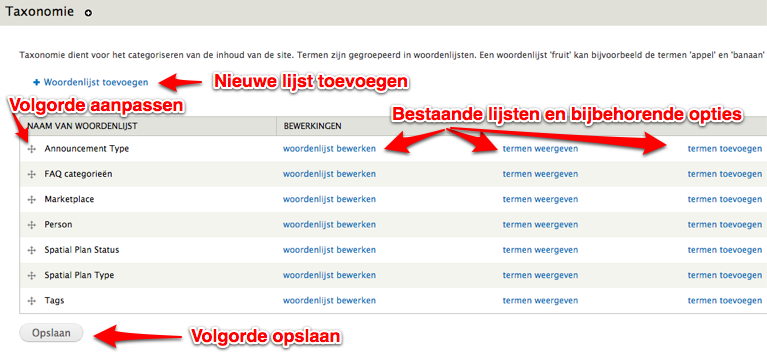
\includegraphics[width=\textwidth]{img/taxonomie2.png}
\end{center}

\subsubsection{Woorden aan woordenlijsten toevoegen}

Ga naar het overzicht van alle woordenlijsten. Klik op 'Termen toevoegen' bij de lijst waaraan je woorden wil toevoegen. Vul bij het veld 'Naam' het woord in en vul eventueel een beschrijving in. Klik onderaan de pagina op de knop 'Opslaan' om het woord aan de lijst toe te voegen. Herhaal deze stappen om meerdere woorden toe te voegen aan de woordenlijst. 

\subsubsection{Woorden in woordenlijsten bewerken}

Het is mogelijk om specifieke woorden uit lijsten te bewerken. Klik op 'Termen weergeven' bij de betreffende lijst.
Klik op 'Bewerken' bij het betreffende woord, vervolgens kun je de wijzigingen doorvoeren. Klik op de knop 'Opslaan' om de wijzigingen op te slaan.

\subsubsection{Woorden uit woordenlijsten verwijderen}

Het is mogelijk om specifieke woorden uit lijsten te verwijderen. Klik op 'Termen weergeven' bij de betreffende lijst.
Klik op 'Bewerken' bij het betreffende woord, om het woord te verwijderen klik je onderaan de op de knop 'Verwijderen'. Na het bevestigen zal het woord definitief en onherstelbaar verwijderd worden.
